% This text is proprietary.
% It's a part of presentation made by myself.
% It may not used commercial.
% The noncommercial use such as private and study is free
% May 2007
% Author: Sascha Frank 
% University Freiburg 
% www.informatik.uni-freiburg.de/~frank/
%
% 
\documentclass{beamer}
\usepackage[latin1]{inputenc}
\usepackage[brazil]{babel}



%Temas
\usetheme[compress]{Dresden}
%\useoutertheme[subsection=false]{smoothbars}
%\useinnertheme[shadow]{rounded}
\useinnertheme{rectangles}


\makeatletter
\beamer@theme@subsectionfalse
\makeatother

\usebackgroundtemplate{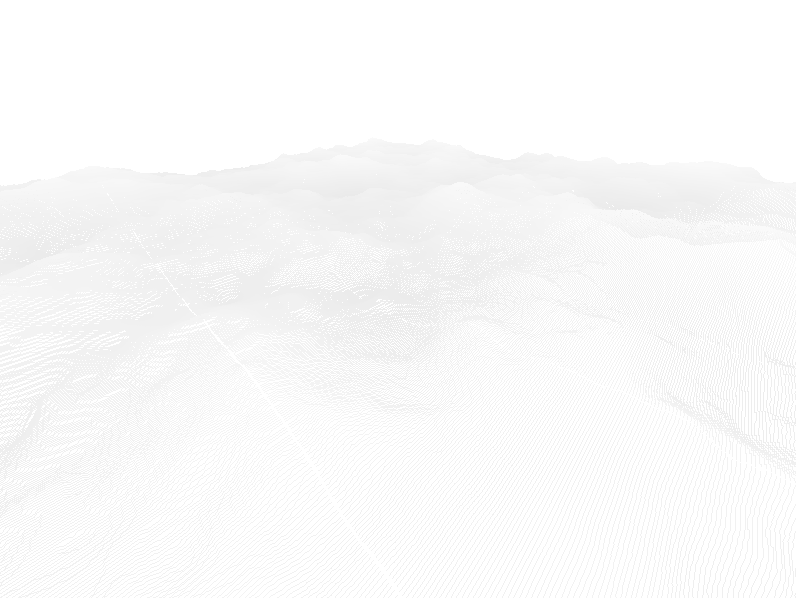
\includegraphics[width=\paperwidth]{img/fundo}}





\begin{document}
\title[Gera��o Procedural de Terrenos em Tempo-Real]{Desenvolvimento de um Arcabou�o para a Gera��o Procedural e Visualiza��o de Terrenos em Tempo-Real}
\author[F�bio Miranda - Apresenta��o final - POC I]{F�bio Markus Nunes Miranda\\Orientador: Prof. Luiz Chaimowicz\\Co-Orientador: Carl�cio Cordeiro}
\institute[Universidade Federal de Minas Gerais]{Departamento de Ci�ncia da Computa��o\\Universidade Federal de Minas Gerais}
\date[\today]{Apresenta��o final - POC I}

\begin{frame}
\titlepage
\end{frame}


\AtBeginSection[]
{
\begin{frame}
\frametitle{Sum�rio}
\setcounter{tocdepth}{1}
\tableofcontents[currentsection]
\setcounter{tocdepth}{2}
\end{frame}
}






\section{Motiva��o}

\subsection{Motiva��o}

\begin{frame}\frametitle{Motiva��o} 
\begin{itemize}
	\item Atualmente, h� uma necessidade de se criar modelos 3D cada vez maiores e com grande n�vel de detalhe.
	\item Por�m, quanto maior e mais detalhado o modelo, mais tempo ter� que ser gasto por um modelador para faz�-lo.
	\item A� entra a gera��o procedural...
\end{itemize}	
\end{frame}

\subsection{Gera��o Procedural}

\begin{frame}\frametitle{O que � gera��o procedural?} 
\begin{itemize}
	\item Gera��o procedural � um termo gen�rico para descrever algoritmos que determinam caracter�sticas de efeitos ou modelos.
	\item H� diversos tipos de t�cnicas e algoritmos, cada um aplicado a uma determinada �rea:
	\begin{itemize}
		\item L-System: gera��o de �rvores e cidades.
		\item Fractais e Perlin Noise: gera��o de terrenos e texturas
	\end{itemize}
\end{itemize}
\end{frame}


%\begin{frame}\frametitle{Gera��o Procedural X Entradas do Usu�rio}
%\begin{itemize}
%	\item Quanto menor o n�mero de entradas do usu�rio, maior o n�vel de gera��o procedural.
%\end{itemize}
%\begin{center}
%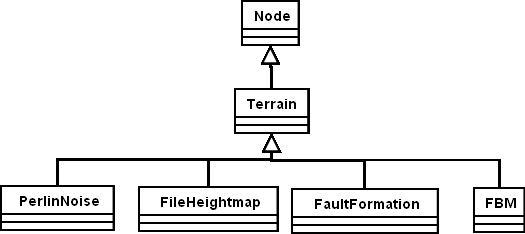
\includegraphics[width=0.5\linewidth]{img/node}
%\end{center}
%\end{frame}



\begin{frame}\frametitle{Vantagens da gera��o procedural} 
\begin{itemize}
	\item Flexibilidade: alterando os par�metros do algoritmo, � poss�vel gerar um grande n�mero de modelos.
	\item Espa�o: n�o h� necessidade de um grande espa�o em disco, j� que tudo ser� ditado por algoritmos.
\end{itemize}
\end{frame}

\begin{frame}\frametitle{Exemplos}
\begin{columns}
	\begin{column}{5cm}
	\begin{itemize}
		\item \alert<1>{.kkrieger\\} \only<1>{\scriptsize Praticamente tudo gerado proceduralmente}
		\item \alert<2>{Elite (1984)\\} \only<2>{\scriptsize Oito gal�xias, 256 planetas.}
		\item \alert<3>{SpeedTree\\} \only<3>{\scriptsize �rvores geradas proceduralmente.}
	\end{itemize}
	\vspace{3cm} 
	\end{column}
	\begin{column}{5cm}
	\begin{overprint}
		\includegraphics<1>[width=1.0\linewidth]{img/kkrieger}
		\includegraphics<2>[width=1.0\linewidth]{img/elite}
		\includegraphics<3>[width=1.0\linewidth]{img/speedtree}
	\end{overprint}
	\end{column}
\end{columns}
\end{frame}

\begin{frame}\frametitle{GPU} 
\begin{itemize}
	\item As atuais placas de v�deo possuem \emph{GPUs} com milhares de unidades de processamento.
	\item Constru�das de forma a processar da melhor maneira poss�vel um grande n�mero de dados independentes entre si, como � o caso de v�rtices e \emph{pixels}.
\end{itemize}
\begin{center}
	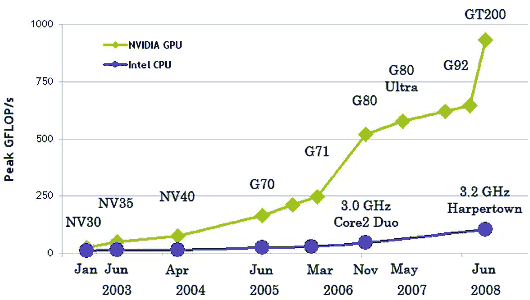
\includegraphics[width=0.5\linewidth]{img/gflops}
\end{center}
\end{frame}


\section{Metodologia}

\subsection{Metodologia}

\begin{frame}\frametitle{Metodologia} 
\begin{itemize}
	\item Livro \emph{Texturing and Modeling: A Procedural Approach} \cite{livro}.
	\item Estudo das melhoras formas de reduzir o gasta com mem�ria atrav�s de estruturas de dados do OpenGL.
	\item Estudo da arquitetura da \emph{GPU}.
	\item Implementa��o do sistema.
\end{itemize}
\end{frame}

\section{Proposta}
\label{proposta}

O terreno geral � dividido em terrenos menores (chamados \emph{patchs}), como mostra o \emph{grid} da Figura \ref{fig:resultados:grid}. Dessa forma, apenas \emph{patchs} de interesse do usu�rio (que est�o mais pr�ximos, por exemplo) precisar�o ser gerados.

\begin{figure}[h]
	\center{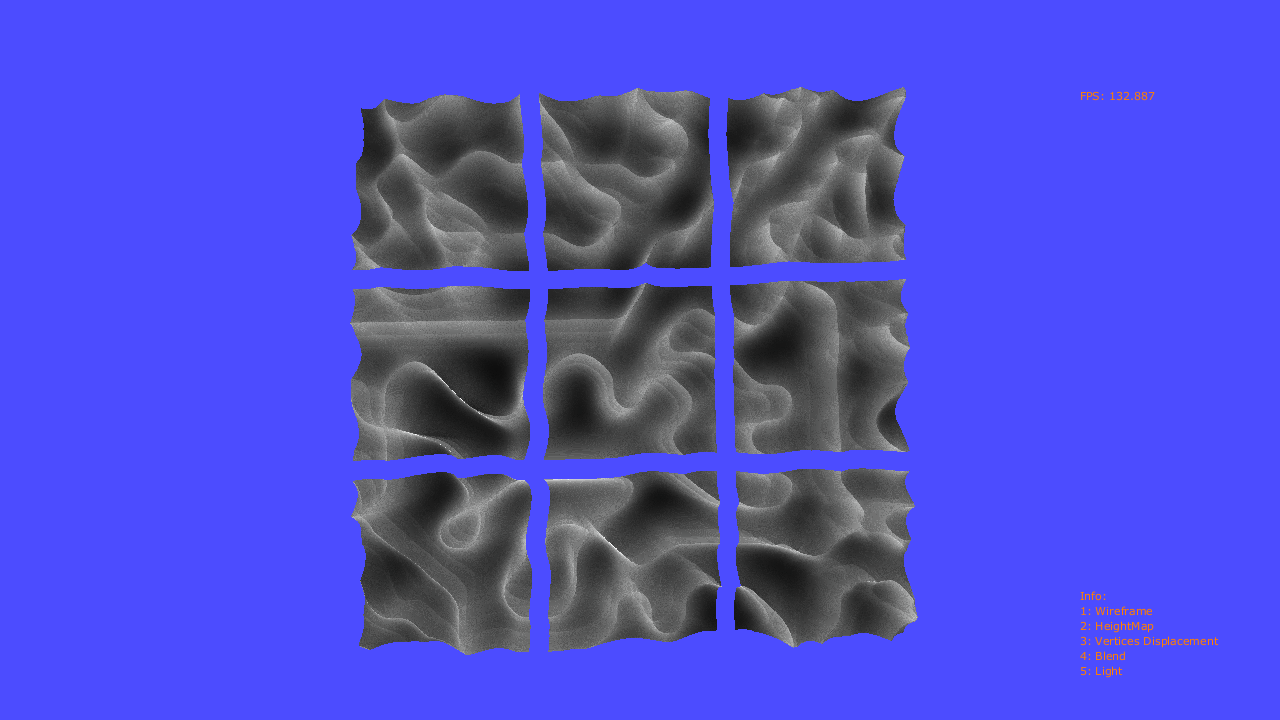
\includegraphics[width=0.6\linewidth]{img/caps/grid.png}}
	\caption{\label{fig:resultados:grid} \emph{Patchs} exibidos em um \emph{grid}.}
\end{figure}

Considerando o usu�rio inicialmente localizado no \emph{patch} central, ao mover-se para um \emph{patch} vizinho, o sistema ir� requisitar a gera�a� de novos \emph{patchs}, vizinhos a aqueles que est�o na borda do grid. O n�mero de vizinhos gerados, bem como a quantidade de vizinhos do \emph{patch} central s�o vari�veis do sistema, podendo ser adaptadas, pelo usu�rio, de acordo com o poder de processamento de sua m�quina.

Para garantir uma visualiza��o fluida do terreno, minimizando as interrup��es com a gera��o, o sistema proposto decidir� qual arquitetura (GPU ou CPU) ser� utilizada na gera��o dos \emph{patchs} a partir de uma vari�vel $\alpha$, que representa a porcentagem de gera��es que ocorrer�o na \emph{GPU}. $1 - \alpha$ representar�, portanto a porcentagem de gera��es na \emph{CPU}.

A Figura \ref{fig:geracao} mostra como se d� o fluxo de gera��o.

\begin{figure}[h]
	\center{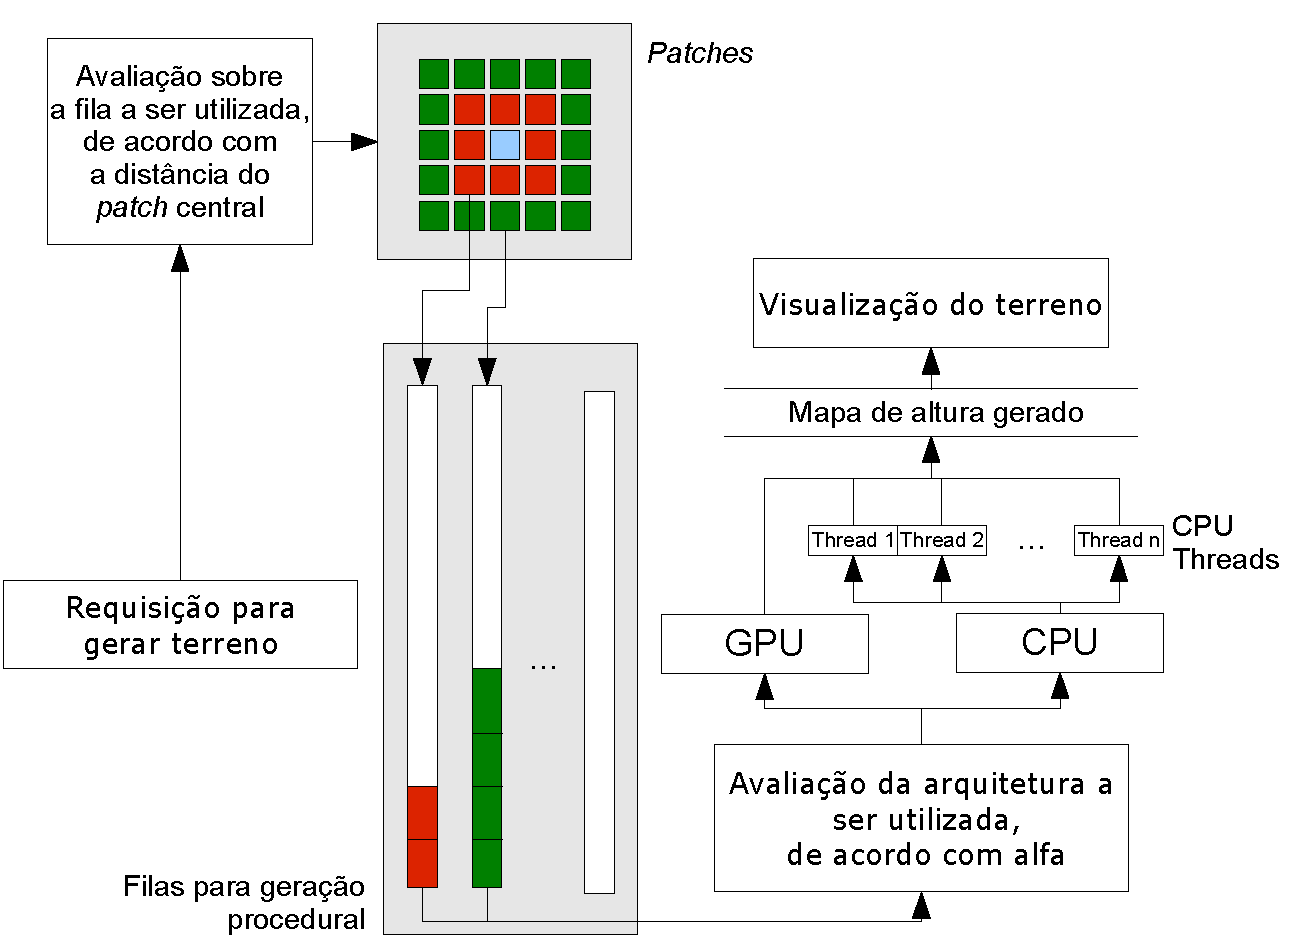
\includegraphics[width=1.0\linewidth]{img/geracao.pdf}}
	\caption{\label{fig:geracao} Fluxo da gera��o procedural.}
\end{figure}


As requisi��es por novos terrenos ser�o adicionadas a uma fila e uma pol�tica \emph{First In, First Out} (FIFO) ser� utilizada para decidir qual terreno ser� gerado. Como � poss�vel ver na Figura \ref{fig:geracao}, o n�mero de filas existentes no sistema ser� igual ao n�mero de vizinhos do \emph{patch} central. Dessa forma, � poss�vel decidir quais terrenos ser�o gerados a partir de sua dist�ncia do \emph{patch} central.

A \emph{thread} principal ficar� encarregada da requisi��o para gerar novos eventos, avalia��o da fila, avalia��o da arquitetura a ser utilizada as chamadas �s fun��es OpenGL. A gera��o na CPU ocorrer� em outras \emph{threads}, n�o a principal.



\subsection{O C�lculo de $\alpha$}

O valor da vari�vel $\alpha$ �, atualmente, uma vari�vel controlada manualmente pelo usu�rio.  A sua varia��o de acordo com a utiliza��o de cada arquitetura ser� um tema a ser abordado em trabalhos futuros.

Atualmente, a maior dificuldade para medir o tempo de gera��o tanto na GPU � a falta de um padr�o nas extens�es dispon�veis em OpenGL. A extens�o \textbf{GL\_EXT\_timer\_query} \cite{timerQuery}, por exemplo, s� est� dispon�vel em placas NVidia, algo que anularia a possibilidade da execu��o deste trabalho em placas ATI.

A utiliza��o de chamadas como \textbf{glFinish()} para sincronizar a CPU e a GPU e assim medir o tempo de gera��o dos terrenos poderia prejudicar a performance do sistema, j� que p�ra a execu��o da CPU enquanto todos os os comandos OpenGL n�o forem executados.

Uma outra op��o para a sincroniza��o seria a extens�o \textbf{GL\_NV\_fence} \cite{nvFence}, que oferece fun��es para sincroniza��o semelhantes ao \textbf{glFinish()} e \textbf{glFlush()}, por�m com um grau maior de controle sobre quais comandos OpenGL dever�o ser executados na chamada. Mais uma vez, por�m, a extens�o n�o est� dispon�vel para placas ATI.

\subsection{Gera��o}
Toda a gera��o dos terrenos na GPU � feita atrav�s de um \emph{fragment shader}, utilizando o ru�do Perlin como foi proposto em \cite{improvedPerlinNoise}. Como toda computa��o de \emph{shaders} fica limitada a geometrias ou texturas, foi preciso renderizar um quadrado utilizando as fun��es OpenGL, para que, dessa forma, fosse poss�vel aplicar os \emph{shaders} �s suas primitivas e iniciar os c�lculos necess�rios. O resultado da gera��o � renderizado em um \emph{framebuffer} \emph{off-screen}, que n�o � exibido na tela, atrav�s da exten��o FBO, que permite criar novos \emph{buffers}.

O c�lculo dos vetores gradientes, necess�rio no ru�do Perlin, � feito na CPU, apenas no in�cio do sistema, e depois � acessado no \emph{fragment shader} como uma textura 2D.

Como o mapa de altura � gerado na GPU, n�o h� qualquer tipo de perda de desempenho com a transfer�ncia entre a mem�ria RAM e a mem�ria da placa de v�deo. Um aspecto importante � que, durante a gera��o do mapa de altura, os valores das normais de cada v�rtice tamb�m s�o calculados.

A gera��o utilizando a CPU � feita utilizando o mesmo algoritmo implementado na GPU. Como o mapa de altura gerado reside na mem�ria principal, sua renderiza��o depender� da transfer�ncia para a mem�ria da placa de v�deo.


\subsection{Visualiza��o}
Com o mapa de altura gerado, o pr�ximo passo � exibir o terreno para o usu�rio, que � feito de forma id�ntica tanto para os terrenos gerados na GPU quanto para os gerados na CPU.

O passo inicial � a gera��o de uma malha (conjunto de v�rtices) de tamanho pr�-determinado, como mostra a Figura \ref{fig:malha}.

\begin{figure}[h]
	\center{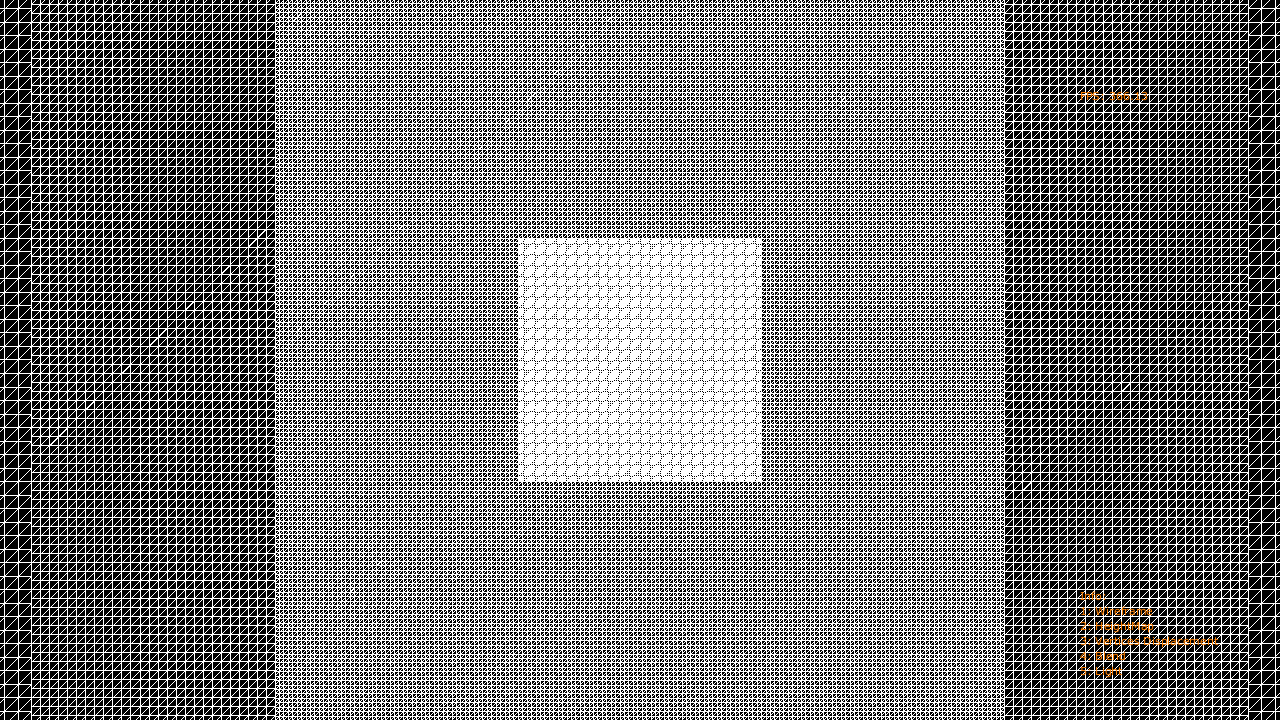
\includegraphics[width=0.5\linewidth]{img/caps/malha.png}}
	\caption{\label{fig:malha} Malha inicial para visualiza��o dos terrenos.}
\end{figure}

A malha � gerada de tal forma que um n�mero maior de v�rtices est� concentrado no centro. Quanto maior a dist�ncia, menor o n�mero de v�rtices presentes. Isto propicia uma maneira r�pida e f�cil de implementar um n�vel de detalhamento (quanto maior a dist�ncia do centro, menor ser� a necessidade de se renderizar o terreno em alta fidelidade).

Como a malha � gerada apenas uma �nica vez (no in�cio da execu��o), n�o � preciso criar repetidas malhas a medida que o jogador percorre o terreno. Apenas os mapas de altura de cada \emph{patch} s�o trocados, como mostra a Figura \ref{fig:texturas}

\begin{figure}[h]
	\center{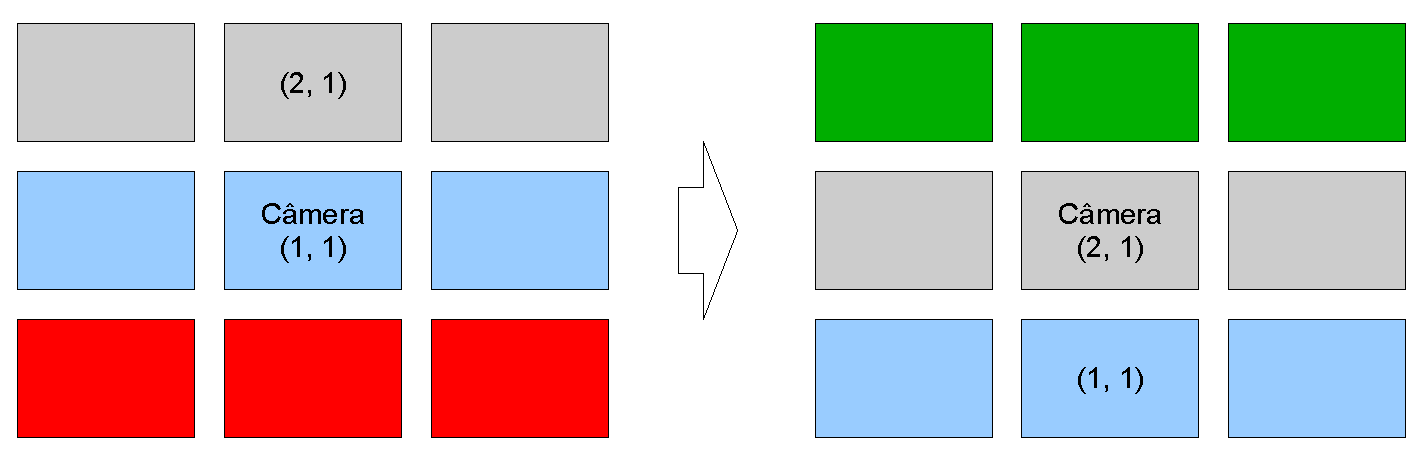
\includegraphics[width=0.8\linewidth]{img/texturas.pdf}}
	\caption{\label{fig:texturas} Movimenta��o da c�mera para um outro \emph{patchs}.}
\end{figure}

Na Figura \ref{fig:texturas} � poss�vel notar o deslocamento dos mapas de textura quando a c�mera move para o \emph{patch} superior ao (1,1). Para que haja uma transi��o, uma matriz de transla��o, com valores iguais ao tamanho do \emph{patch}, � feita e multiplicada � matriz respons�vel por renderizar todas as primitivas, resultando na transla��o de todos os \emph{patchs}. 

Este m�todo diminuiu a necessidade de implementa��o de um algoritmo de n�vel de detalhe mais robusto. Al�m disso, como sabemos o n�mero de v�rtices antecipadamente, a performance do aplicativo tem uma menor chance de sofrer quedas bruscas de rendimento.


\chapter{RESULTADOS E DISCUSS�O}
\label{resultados}
Neste cap�tulo, ser� apresentado algumas imagens de terrenos gerados (Se��o \ref{terrenosgerados}) e tamb�m algum testes executados (\ref{testes}).


\section{Terrenos gerados}
\label{terrenosgerados}

A Figura \ref{fig:heightmap2} mostra a renderiza��o de uma cena apenas com a textura do mapa de altura aplicado em um quadrado.
\begin{figure}[H]
	\center{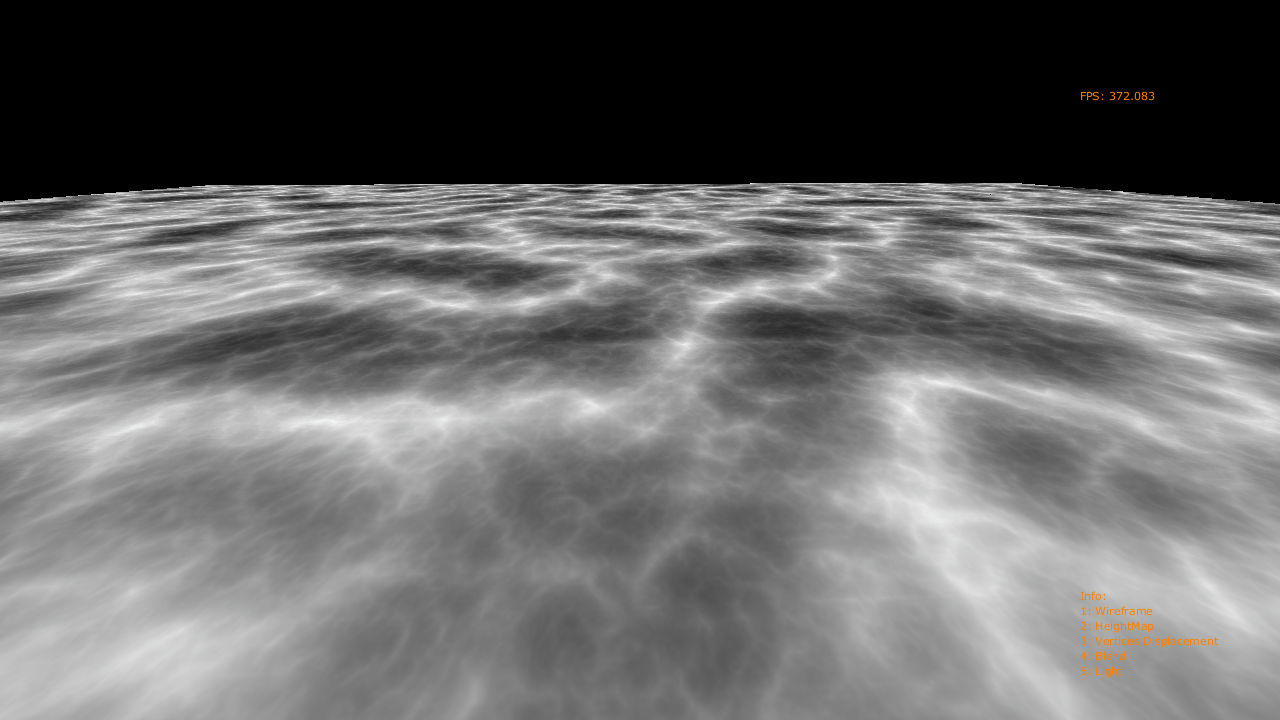
\includegraphics[width=0.5\linewidth]{img/caps/heightmap2.png}}
	\caption{\label{fig:heightmap2} Mapa de altura aplicado a um quadrado.}
\end{figure}


A Figura \ref{fig:deslocamento} mostra o mesmo mapa de altura, mas agora com o deslocamento dos v�rtices no eixo \emph{z}.
\begin{figure}[H]
	\center{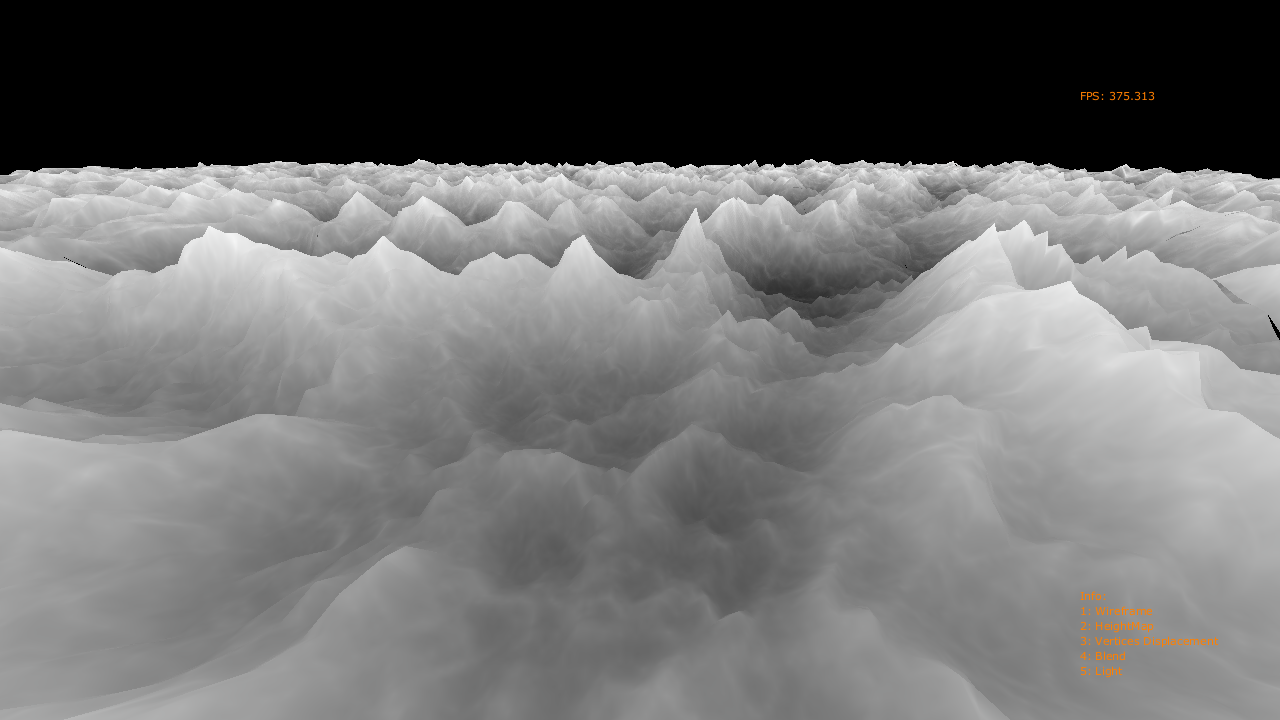
\includegraphics[width=0.5\linewidth]{img/caps/deslocamento.png}}
	\caption{\label{fig:deslocamento} Mapa de altura aplicado a um quadrado, deslocando a altura.}
\end{figure}

A Figura \ref{fig:blend} mostra agora a renderiza��o da malha com cores para simular grama, pedras, neve, etc.
\begin{figure}[H]
	\center{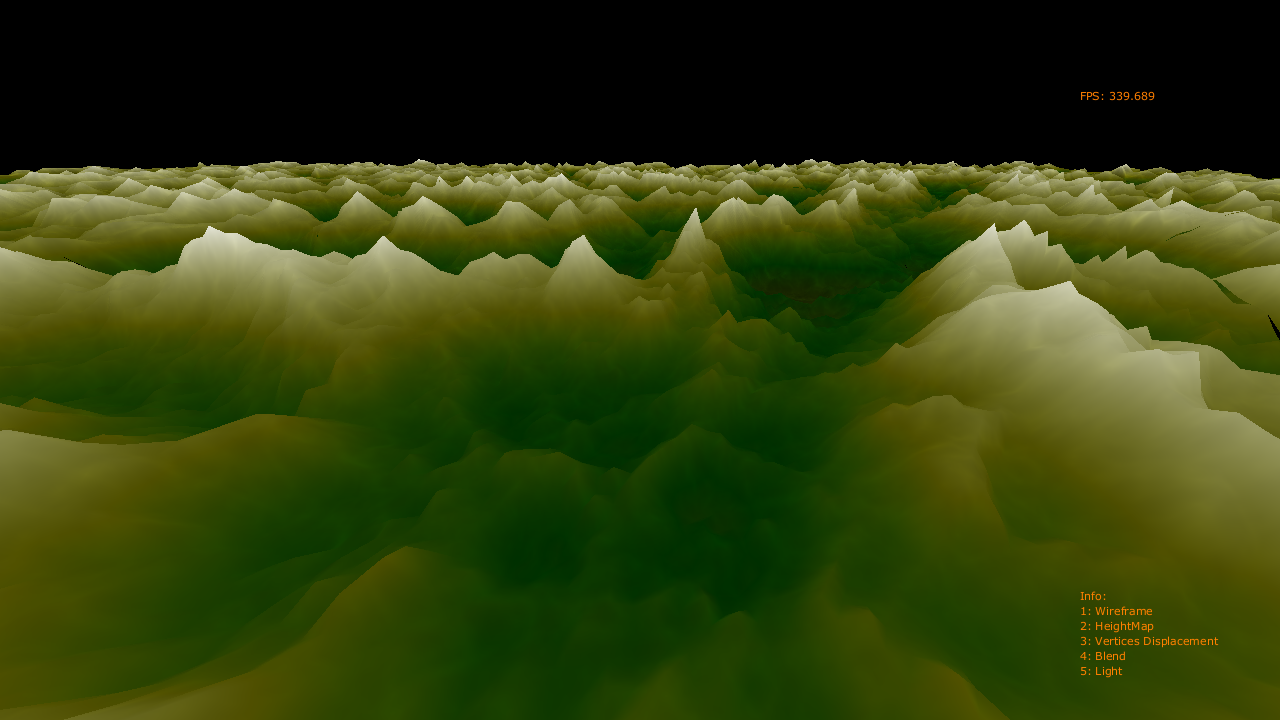
\includegraphics[width=0.5\linewidth]{img/caps/blend.png}}
	\caption{\label{fig:blend} Mapa de altura aplicado a um quadrado, deslocando a altura, e com texturas.}
\end{figure}

A Figura \ref{fig:luz} mostra o resultado final, agora com a aplica��o de ilumina��o.
\begin{figure}[H]
	\center{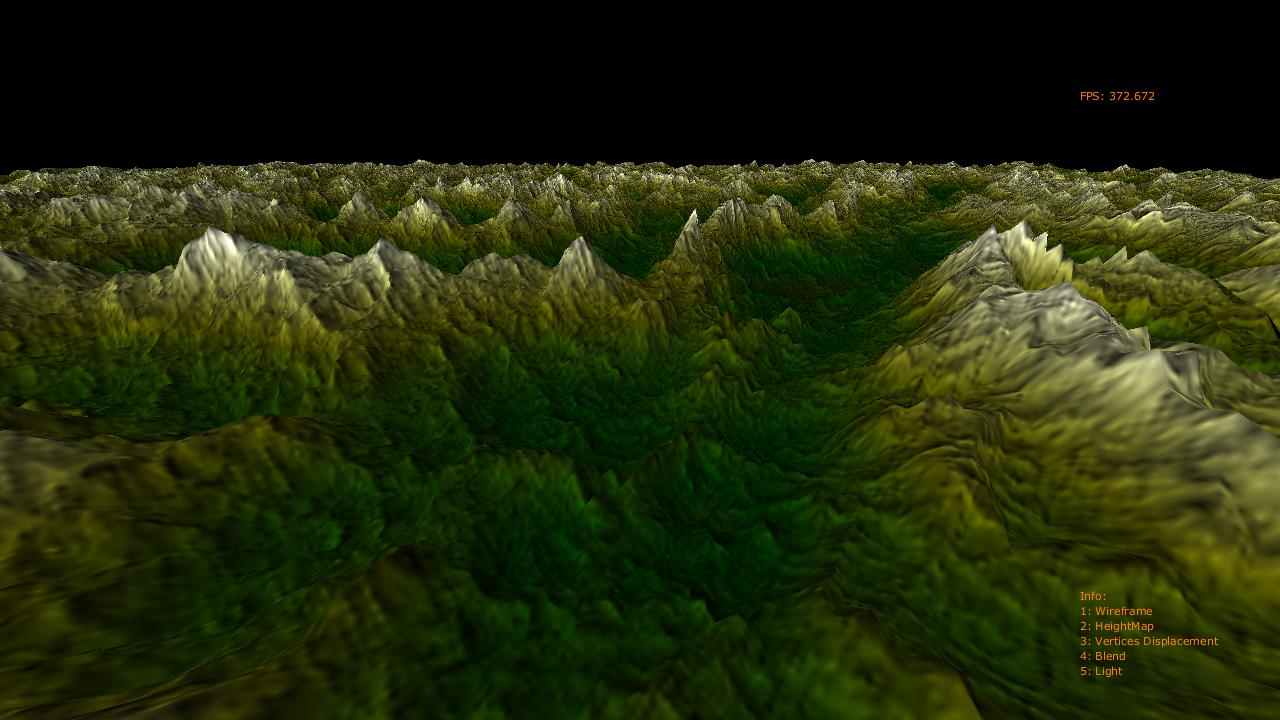
\includegraphics[width=0.5\linewidth]{img/caps/luz.png}}
	\caption{\label{fig:luz} Mapa de altura aplicado a um quadrado, deslocando a altura, com texturas, e ilumina��o.}
\end{figure}

Um v�deo demonstrando a navega��o pelo terreno pode ser visto em \cite{youtube}.


\section{Testes de Desempenho}
\label{testes}
Alguns testes foram feitos para avaliar a velocidade de gera��o dos terrenos com a altera��o de alguns par�metros, utilizando tanto a GPU quanto a CPU. Eles foram executados em um \emph{Core 2 Duo E7400}, com 2GB de mem�ria \emph{RAM} e placa de v�deo \emph{ATI Radeon HD 4850} com 512MB de mem�ria \emph{RAM}, e \emph{driver} vers�o 8.612. As tabelas com os tempos e as conclus�es dos testes s�o apresentadas a seguir.



\subsection{Tempos de Gera��o do Terreno}
\label{testeGeracao}
Neste teste foi medido o tempo m�dio gasto com a gera��o de terrenos tanto na \emph{GPU} quanto na \emph{CPU}. Os seguintes par�metros foram utilizados:

\begin{itemize}
\item \emph{Octaves}: Vari�vel (4, 8, 12, 16)
\item \emph{Lacunarity}: 2.5
\item Ganho: 0.5
\item \emph{Offset}: 1.0
\item Tamanho da textura: 512
\item N�mero de divis�es dos quadrados: 150
\item Tamanho dos quadrados: 5.0
\item Fator \emph{LOD}: 2
\end{itemize}



\begin{table}[H]
	\begin{center}
		\begin{tabular}{|c|c|c|}
			\hline
			\emph{Octaves} & GPU & CPU \\
			\hline
			4 & 28,7236 & 46,2948\\
			\hline
			8 & 28,7432 & 92,4299\\
			\hline
			16 & 28,7887 & 187,103\\
			\hline
			32 & 30,1095 & 370,841\\
			\hline
		\end{tabular}
		\caption{Tempo m�dio (em ms) de gera��o dos terrenos, com n�mero vari�vel de \emph{octaves}}
		\label{tabela:geracao}
	\end{center}
\end{table}


A Figura \ref{fig:geracao} apresenta os tempos anteriores.
\begin{figure}[H]
	\center{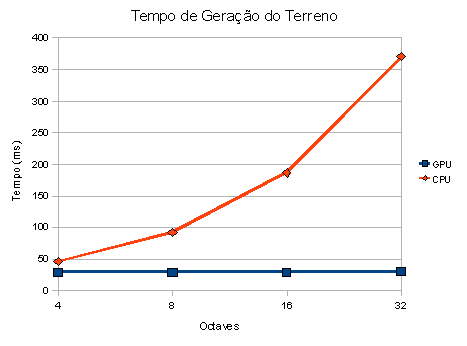
\includegraphics[width=0.4\linewidth]{img/tempoGeracao.png}}
	\caption{\label{fig:geracao} Gr�fico do tempo m�dio (em ms) de gera��o dos terrenos, com n�mero vari�vel de \emph{octaves}.}
\end{figure}


Como pode ser visto, o tempo de gera��o do terreno na \emph{GPU} permanece quase constante, enquanto a gera��o na \emph{CPU} tem um comportamento praticamente linear.


\subsection{\emph{Frames} por Segundo Durante Navega��o}
\label{testeFPS}
Neste teste foi medido o \emph{Frames por segundo} (\sigla{FPS}{Frames por segundo}) m�dio durante a navega��o pelo terreno gerado proceduralmente, por 30 segundos. Os seguintes par�metros foram utilizados:

\begin{itemize}
\item \emph{Octaves}: 16
\item \emph{Lacunarity}: 2.5
\item Ganho: 0.5
\item \emph{Offset}: 1.0
\item Tamanho da textura: 512
\item N�mero de divis�es dos quadrados: 150
\item Tamanho dos quadrados: 5.0
\item Fator \emph{LOD}: 2
\end{itemize}

A Tabela \ref{tabela:fps} mostra os tempos m�dios, m�nimos e a m�dia de \emph{FPS}. Al�m disso, h� o n�mero de \emph{frames} renderizados durante o percurso:

\begin{table}[H]
	\begin{center}
		\begin{tabular}{|c|c|c|c|c|}
			\hline
			 & Total de \emph{Frames} & \emph{FPS} M�nimo & \emph{FPS} M�ximo & \emph{FPS} M�dio \\
			\hline
			CPU & 9664 & 248 & 397 & 322.133\\
			\hline
			GPU & 11287 & 361 & 394 & 376.233\\
			\hline
		\end{tabular}
		\caption{Dados sobre a navega��o pelo mundo durante 30 segundos}
		\label{tabela:fps}
	\end{center}
\end{table}


A Figura \ref{fig:fps} apresenta os tempos anteriores:
\begin{figure}[H]
	\center{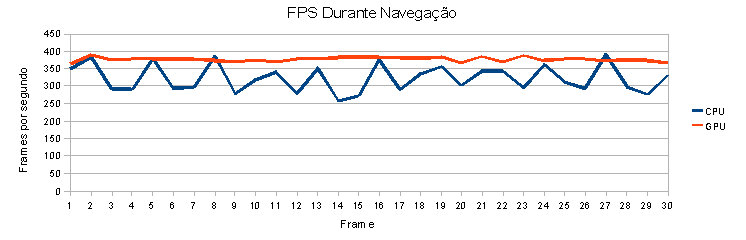
\includegraphics[width=0.9\linewidth]{img/tempoFPS.png}}
	\caption{\label{fig:fps} Gr�fico com o FPS na navega��o pelo mundo durante 30 segundos.}
\end{figure}


Como pode ser visto atrav�s do gr�fico, a navega��o pelo mundo, utilizando a gera��o dos terrenos na GPU, � muito mais fluida, sem quedas bruscas de \emph{FPS}, como nos \emph{frames} 3, 6, 9, 12, 14, 17, 20, 23, 26 e 29, gra�as �s centenas de unidades de processamento presentes na GPU.

Na gera��o pela CPU, tais quedas correspondem justamente aos momentos em que o sistema gera novos terrenos e podem significar um menor senso de imers�o do usu�rio no mundo virtual.


\chapter{CONCLUS�ES E TRABALHOS FUTUROS}
\label{conclusao}

%O trabalho desenvolvido em POC I teve como objetivo principal estabelecer uma base para ser desenvolvida posteriormente em POC II, e tamb�m como uma forma de aprendizado de t�cnicas procedurais. A intera��o do usu�rio com o terreno gerado ser� aprofundada ainda mais, permitindo a inser��o n�o s� de mapas de altura, mas tamb�m de modelos tridimensionais, como, por exemplo, casas.

%Um ponto a ser otimizado � a c�pia dos v�rtices para as estruturas VBO. Dessa forma, ser� poss�vel diminuir o tempo total gasto com a gera��o procedural dos terrenos, e suavizar as transi��es entre terrenos. Outro ponto que pode ser abordado � a visualiza��o dos terrenos na medida em que eles s�o gerados; no caso do ru�do de Perlin, a visualiza��o poderia ser a cada \emph{octave} gerado. Terrenos mais longe da c�mera poderiam tamb�m ser gerados com um n�mero menor de \emph{octaves}. Al�m disso, o processamento em paralelo pode ser explorado, um dos temas abordados no paradigma apresentado em \cite{carlucio}.

%O uso de texturas tamb�m ser� aprofundado, possivelmente com o uso de sombras pr�-calculadas \cite{slopelighting}. Outra quest�o a ser desenvolvida em POC II � uma \emph{interface} gr�fica mais atrativa, e uma forma eficiente de se armazenar as informa��es inseridas pelo usu�rio, possivelmente em arquivos \emph{Extensible Markup Language} (\sigla{XML}{Extensible Markup Language}).

Os resultados obtidos na gera��o procedural de terrenos na GPU mostram o poder de processamento das placas gr�ficas, em rela��o �s CPU. Este trabalho, por�m, n�o implementou uma alternativa \emph{multi-core} para a gera��o procedural na CPU. Isto poderia diminuir o tempo gasto na gera��o. Outro aspecto que pode ser abordado no futuro � o escalonamento entre GPU e CPU, dependendo do n�vel de ociosidade de cada processador.

Um ponto a ser melhorado na gera��o procedural � quanto � heterogeneidade do terreno. Apesar de apresentar um resultado satisfat�rio para um local limitado, quando se olha o terreno como um todo, percebe-se que h� uma semelhan�a muito grande entre os \emph{patchs}, diminuindo assim a ilus�o de estar andando em algo realmente infinito.

O sistema foi implementado sempre tendo em mente a sua utiliza��o acoplada a outras aplicativos. Dessa forma, adot�-lo em um simulador ou \emph{game} demandaria pouco esfor�o, desde que o aplicativo utilize \emph{OpenGL}.


\section{Bibliografia}
\begin{tiny}
\nocite{*}
\bibliographystyle{unsrt}
\bibliography{apresentacao_monografia}
\end{tiny}


\begin{frame}
\Large D�vidas?
\end{frame}




\end{document}
